%-----------------------------------------------------------------%
% 2015 - 2023 Emerson Ribeiro de Mello - mello@ifsc.edu.br
% 
% 2023/04/10 versão 1.01
% 
% Modelo de monografia para o Instituto Federal de Santa Catarina
% 
% Adaptação do documento abnTeX2: Modelo de Trabalho Acadêmico
% para ficar de acordo com o "Template para elaboração de trabalho 
% acadêmico" fornecido pela Biblioteca do IFSC 
% https://www.ifsc.edu.br/documentos-uteis. Acesso em 2022-08-27
% 
%-----------------------------------------------------------------%
\documentclass[
	12pt,				% tamanho da fonte
	openright,			% capítulos começam em pág ímpar (insere página vazia caso preciso)
	twoside,			% para impressão em recto e verso. Oposto a oneside
	a4paper,			% tamanho do papel. 
	% -- opções da classe abntex2 --
	chapter=TITLE,		% títulos de capítulos convertidos em letras maiúsculas
	english,			% idioma adicional para hifenização
	% french,				% idioma adicional para hifenização
	% spanish,			% idioma adicional para hifenização
	brazil				% o último idioma é o principal do documento
	]{ifscthesis}


%-----------------------------------------------%
% Capa
%-----------------------------------------------%

%-----------------------------------------------%
% Para alterar o gênero dos comandos orientador
% e coorientador.
%-----------------------------------------------%
% \renewcommand{\orientadorname}{Orientadora:}
\renewcommand{\coorientadorname}{Coorientadora:}
%-----------------------------------------------%


%-----------------------------------------------%
% Informações de dados para CAPA e FOLHA DE ROSTO
%-----------------------------------------------%
\titulo{Modelo de Trabalho Acadêmico com \abnTeX}
\autor{Nome do Aluno}
\local{São José - SC}
\data{agosto/2022}
\orientador{Prof. Orientador da Silva, Dr.}
\coorientador{Profa. Fulana da Silva, Dra.}
\instituicao{%
  Instituto Federal de Santa Catarina -- IFSC
  \par
  Campus São José
  \par
  Engenharia de Telecomunicações}
\tipotrabalho{Monografia (Graduação)}
%-----------------------------------------------%




%-----------------------------------------------%
% O preambulo deve conter o tipo do trabalho, o objetivo, o nome da instituição e a área de concentração 
\preambulo{Monografia apresentada ao Curso de Engenharia de Telecomunicações do campus São José do Instituto Federal de Santa Catarina para a obtenção do diploma de Engenheiro de Telecomunicações.}

\textoaprovacao{Este trabalho foi julgado adequado para obtenção do título de Engenheiro de Telecomunicações, pelo Instituto Federal de Educação, Ciência e Tecnologia de Santa Catarina, e aprovado na sua forma final pela comissão avaliadora abaixo indicada.}
%-----------------------------------------------%

%-----------------------------------------------%
% Estilo de cabeçalho que só contém o número da 
% página e uma linha
%-----------------------------------------------%
\makepagestyle{cabecalholimpo}
\makeevenhead{cabecalholimpo}{\thepage}{}{} % páginas pares
\makeoddhead{cabecalholimpo}{}{}{\thepage} % páginas ímpares
% \makeheadrule{cabecalholimpo}{\textwidth}{\normalrulethickness} % linha
%-----------------------------------------------%


%-----------------------------------------------%

%-----------------------------------------------%
% Incluir arquivo com acrônimos e símbolos
%-----------------------------------------------%
% 
% ATENÇÃO. Este projeto faz uso do pacote glossaries.
% Se for usar uma instalação local do LaTeX para
% compilar, e não no Overleaf, então é necessário 
% que tenha o arquivo .latexmkrc dentro diretório 
% deste projeto e use o comando abaixo:
% 
% latexmk -outdir=out -pdf monografia.tex
% 
% A extensão LaTeX Workshop do Visual Studio Code
% usa por padrão o latexmk para compilar
\makeglossaries


\newacronym
{json} % rótulo 
{JSON} % sigla
{\textit{JavaScript Object Notation}} % por extenso

\newacronym{ABNT}{ABNT}{Associação Brasileira de Normas Técnicas}

\newacronym{abnTeX}{abnTeX}{ABsurdas Normas para TeX}

\newacronym[longplural={Autoridades Certificadoras}]{AC}{AC}{Autoridade Certificadora}

\newacronym{AES}{AES}{\textit{Advanced Encryption Standard}}

\newacronym{TLS}{TLS}{\textit{Transport Layer Security}}

\newacronym{TPC}{TPC}{Terceira Parte Confiável}

\newacronym{IFSC}{IFSC}{Instituto Federal de Santa Catarina}
\glsxtrnewsymbol[description={conjunto vazio}]
{emptyset}% rótulo (será usado na ordenação na lista de símbolos)
{\ensuremath{\emptyset}}% símbolo


\glsxtrnewsymbol[description={número Pi}]
{pi}% rótulo (será usado na ordenação na lista de símbolos)
{\ensuremath{\pi}}% símbolo



%-----------------------------------------------%
% Início do documento
%-----------------------------------------------%
\begin{document}
% Seleciona o idioma do documento (conforme pacotes do babel)
\selectlanguage{brazil}




%-----------------------------------------------%
% ELEMENTOS PRÉ-TEXTUAIS
%-----------------------------------------------%
\pretextual
\imprimircapa
%-----------------------------------------------%

%-----------------------------------------------%
% No arquivo abaixo tem detalhes sobre folha de
% aprovação, ficha catalográfica, agradecimentos,
% resumo, abstract, etc.
% 
% Se não for a versão final do PDF, talvez fosse
% interessante comentar a linha abaixo.
%-----------------------------------------------%
%-----------------------------------------------%
% Folha de rosto
% (o * indica que haverá a ficha bibliográfica)
%-----------------------------------------------%
% \imprimirfolhaderosto*
\imprimirfolhaderosto
%-----------------------------------------------%

%-----------------------------------------------%
% ficha bibliográfica
% 
% Pegue com a Biblioteca do IFSC um PDF com a 
% ficha correta, salve o arquivo no diretório
% deste projeto e descomente as linhas abaixo
% \begin{fichacatalografica}
%     \includepdf{ficha-catalografica.pdf}
% \end{fichacatalografica}
%-----------------------------------------------%

%-----------------------------------------------%


%-----------------------------------------------%
% folha de aprovação
%-----------------------------------------------%
\begin{folhadeaprovacao}

    \begin{center}
        {\ABNTEXchapterfont\large\imprimirautor}

        \vspace*{\fill}\vspace*{\fill}
        \begin{center}
            \ABNTEXchapterfont\Large\imprimirtitulo
        \end{center}
        \vspace*{\fill}

        \imprimirtextoaprovacao

        \vspace*{1cm}

        \imprimirlocal, 10 de abril de 2023:

        \vspace*{\fill}
    \end{center}

    % Alterando o espaço para assinatura de 0.7cm para 1.5cm
    \setlength{\ABNTEXsignskip}{1.5cm}

    \assinatura{\textbf{\imprimirorientador} \\ Orientador\\Instituto Federal de Santa Catarina}     
    \assinatura{\textbf{Professor Fulano, Dr.} \\ Instituto Federal de Santa Catarina }
    \assinatura{\textbf{Professora Fulana, Dra. } \\ Instituto Federal de Santa Catarina}
    % \assinatura{\textbf{Professor Beltrano, Dr.} \\ Instituto Z}

    \vspace*{1cm}
  
\end{folhadeaprovacao}
%-----------------------------------------------%


%-----------------------------------------------%
% Dedicatória
%-----------------------------------------------%
\begin{dedicatoria}
    \vspace*{\fill}
    \begin{flushright}
    \noindent
    \textit{ Este trabalho é dedicado às crianças adultas que,\\
    quando pequenas, sonharam em se tornar cientistas.}\vspace*{2cm}
    \end{flushright}
 \end{dedicatoria}

%-----------------------------------------------%


%-----------------------------------------------%
% Agradecimentos
%-----------------------------------------------%
\begin{agradecimentos}
    Os agradecimentos principais são direcionados à Gerald Weber, Miguel Frasson,
    Leslie H. Watter, Bruno Parente Lima, Flávio de Vasconcellos Corrêa, Otavio Real
    Salvador, Renato Machnievscz\footnote{Os nomes dos integrantes do primeiro
    projeto abn\TeX\ foram extraídos de
    \url{http://codigolivre.org.br/projects/abntex/}} e todos aqueles que
    contribuíram para que a produção de trabalhos acadêmicos conforme
    as normas ABNT com \LaTeX\ fosse possível.
    
    Agradecimentos especiais são direcionados ao Centro de Pesquisa em Arquitetura
    da Informação\footnote{\url{http://www.cpai.unb.br/}} da Universidade de
    Brasília (CPAI), ao grupo de usuários
    \emph{latex-br}\footnote{\url{http://groups.google.com/group/latex-br}} e aos
    novos voluntários do grupo
    \emph{\abnTeX}\footnote{\url{http://groups.google.com/group/abntex2} e
    \url{http://www.abntex.net.br/}}~que contribuíram e que ainda
    contribuirão para a evolução do \abnTeX.
\end{agradecimentos}
%-----------------------------------------------%


%-----------------------------------------------%
% Epígrafe
%-----------------------------------------------%
\begin{epigrafe}
    \vspace*{\fill}
    \begin{flushright}
        \textit{Sempre que te perguntarem se podes fazer um trabalho,\\
        respondas que sim e te ponhas em seguida a aprender como se faz.\\
        T. Roosevelt}
    \end{flushright}
\end{epigrafe}
%-----------------------------------------------%


%-----------------------------------------------%
% Resumo e abstract
%-----------------------------------------------%
% ajusta o espaçamento dos parágrafos do resumo
\setlength{\absparsep}{18pt} 
\begin{resumo}
    O resumo deve ressaltar o objetivo, o método, os resultados e as conclusões do documento. A ordem e a extensão destes itens dependem do tipo de resumo (informativo ou indicativo) e do tratamento que cada item recebe no documento original. O resumo deve ser precedido da referência do documento, com exceção do resumo inserido no próprio documento. O resumo deve conter apenas um parágrafo com no mínimo 150 e no máximo 250 palavras. As palavras-chave devem figurar logo abaixo do resumo, antecedidas da expressão Palavras-chave:, separadas entre si por ponto e finalizadas também por ponto. Este documento segue as normas da \gls{ABNT} e para isso faz uso do pacote \gls{abnTeX}.
    
    \textbf{Palavras-chave}: latex. abntex. editoração de texto.
\end{resumo}

%-----------------------------------------------%
\begin{resumo}[Abstract]
\begin{otherlanguage*}{english}
    This is the english abstract.
\vspace{\onelineskip}

\noindent 
\textbf{Keywords}: latex. abntex. text editoration.
\end{otherlanguage*}
\end{resumo}
%-----------------------------------------------%
%-----------------------------------------------%

%-----------------------------------------------%
% Listas ilustrações, tabelas, códigos, abreviaturas
% símbolos.
% Comente a linha abaixo para não gerar as listas
%-----------------------------------------------%

%-----------------------------------------------%
% Listas ilustrações, tabelas, códigos, abreviaturas
% símbolos
%-----------------------------------------------%

% Lista de ilustrações
\pdfbookmark[0]{\listfigurename}{lof}
\listoffigures*
\cleardoublepage

% Lista de quadros
\pdfbookmark[0]{\listofquadrosname}{loq}
\listofquadros*
\cleardoublepage

% Lista de tabelas
\pdfbookmark[0]{\listtablename}{lot}
\listoftables*
\cleardoublepage

% Lista de códigos
\pdfbookmark[0]{\lstlistlistingname}{lol}
\begin{KeepFromToc}
\lstlistoflistings
\end{KeepFromToc}
\cleardoublepage

% Lista de abreviaturas
\printglossary[type=\acronymtype,nonumberlist,title=Lista de abreviaturas e siglas]
\cleardoublepage

% Lista de símbolos
\printglossary[type=symbols,nonumberlist,title=Lista de símbolos]
\cleardoublepage

% Sumário
\pdfbookmark[0]{\contentsname}{toc}
\tableofcontents*
\cleardoublepage
%-----------------------------------------------%


%-----------------------------------------------%
% Elementos textuais - Capítulos
%-----------------------------------------------%
% Se quiser que apareça o título dos capítulos
% no cabeçalho, então comente a linha abaixo
\pagestyle{cabecalholimpo}

\chapter{Introdução}\label{cap:introducao}

A introdução abre o trabalho propriamente dito. Tem a finalidade de apresentar os motivos que levaram o autor a realizar a pesquisa, o problema abordado, os objetivos e a justificativa. O objetivo principal da introdução é situar o leitor no contexto da pesquisa. O leitor deverá perceber claramente o que foi analisado, como e por que, as limitações encontradas, o alcance da investigação e suas bases teóricas gerais. Ela tem, acima de tudo, um caráter didático de apresentar o que foi investigado, levando-se em conta o leitor a que se destina e a finalidade do trabalho. 

Assim, na introdução contextualize o tema, delimite o assunto, apresente um rápido histórico do problema e das soluções porventura já apresentadas, com breve revisão crítica das investigações anteriores; faça referência às fontes de material, aos métodos seguidos, às teorias ou aos conceitos que embasam o desenvolvimento e a argumentação, às eventuais faltas de informação, ao instrumental utilizado. A introdução deverá conter, ainda:

\begin{enumerate}
   \item Justificativa;
   \item Definição do problema;
   \item Objetivo geral e objetivos específicos.
\end{enumerate}

\section{Objetivos}

\subsection{Objetivo geral}

\subsection{Objetivos específicos}


\section{Organização do texto}

O texto está organizado da seguinte forma: No \autoref{cap:revisao} é apresentado um pouco mais de como fazer um outro capítulo, apresentando ainda formas para inserir figuras. No \autoref{cap:proposta} é apresentado uma forma para adicionar uma tabela. Por fim, no \autoref{cap:conclusoes} são apresentadas as conclusões sobre este trabalho.
\chapter{Revisão bibliográfica}\label{cap:revisao}

É uma análise comentada sobre o que já foi publicado sobre o assunto da pesquisa, buscando mostrar os pontos de vista convergentes e divergentes entre os autores. Traça-se um quadro teórico e elabora-se a estruturação conceitual que subsidiará o desenvolvimento da pesquisa. A revisão de literatura permitirá um mapeamento de quem já escreveu e o que já foi escrito sobre o assunto ou o problema de pesquisa.


\section{Quadros}\label{sec:quadros}


Um quadro é formado por linhas horizontais e verticais, sendo fechado em todas as suas extremidades e, geralmente, é utilizado para expressar dados qualitativos. Verifique um exemplo de utilização no \autoref{quadro:exemplo}.


\begin{quadro}[htb]
\caption{Exemplo de quadro}\label{quadro:exemplo}
\begin{tabular}{|l|r|r|r|}
    \hline
    \textbf{Pessoa} & \textbf{Idade} & \textbf{Peso} & \textbf{Altura} \\ \hline
    Marcos & 26    & 68   & 178    \\ \hline
    Ivone  & 22    & 57   & 162    \\ \hline
    ...    & ...   & ...  & ...    \\ \hline
    Sueli  & 40    & 65   & 153    \\ \hline
\end{tabular}
\fonteproprioautor
\end{quadro}

No \autoref{quadro:docentes} são listados os docentes do curso.

\begin{quadro}[htb]
    \centering
    \caption{Listagem dos docentes do curso}\label{quadro:docentes}
    \footnotesize
    \begin{tabular}{|l|l|l|}
    \hline
    \textbf{Docente} & \textbf{Formação acadêmica}    & \textbf{UCs}                               \\ \hline
    Fulano de tal    & Engenharia de Telecomunicações & Antenas, Radiotransmissão, Circuitos de RF \\ \hline
    Nononono         & Ciências da Computação         & Programação, Sistemas Distribuídos         \\ \hline
    Sicrano          & Engenharia Elétrica            & Análise de Circuitos, Sinais e Sistemas    \\ \hline
    \end{tabular}
    \fonteproprioautor
\end{quadro}


\section{Tabelas}\label{sec:tabelas}

De acordo com \citeonline{ibge1993}, tabelas são ilustrações com dados estatísticos numéricos. A moldura de uma tabela não deve ter traços verticais que a delimitem à esquerda e à direita. Quando houver necessidade de se destacar parte do cabeçalho ou parte dos dados numéricos estes devem ser estruturados com um ou mais traços verticais paralelos adicionais. Linhas horizontais só se admitem no cabeçalho e no rodapé. 

Tabelas não devem figurar dados em branco. Assim, em um tabela:

\begin{itemize}
    \item Traço indica dado inexistente;
    \item Reticências indicam dado desconhecido;
    \item Zero deve ser usado quando o dado for menor que a metade da unidade adotada para a expressão do dado.
\end{itemize}

As tabelas devem ser citadas no texto, inseridas o mais próximo possível do trecho a que se referem e padronizadas segundo as Normas de Apresentação Tabular do IBGE. Os números sempre devem ser alinhados à direita, veja um exemplo na \autoref{tab:publicacoes}.

\begin{table}[htb]
    \ABNTEXfontereduzida
    \centering
    \caption{Produção dos docentes do curso}
    \label{tab:publicacoes}
    \begin{tabular}{p{3.3cm} r r R{2cm}}\toprule
        Produto científico & \multicolumn{2}{c}{Período} &  \\ \cmidrule{2-3}
                   & 2000-2010 & 2010-2020 & Total \\ \midrule
        Artigo nacional & 10 & 20 & 30 \\ 
        Artigo internacional & 5 & 5 & 10 \\
        Orientações de TCC & 30 & 40 & 70 \\ \midrule 
        Total & 45 & 65 & 110 \\

        \bottomrule
    \end{tabular}
    \fonteproprioautor
\end{table}



\section{Figuras}\label{sec:figuras}

As figuras são bastante úteis para ajudar expressar o funcionamento, modelo, etc. de alguma parte de seu trabalho. O \textit{Inkscape}\footnote{\url{https://inkscape.org/pt-br}.} é um \textit{software} livre para criação de desenhos vetoriais e que permite exportar os desenhos para os formatos PDF, PNG etc. O \textit{site} \url{https://diagrams.net} também uma boa opção para criar figuras.

A inclusão de figuras no texto necessita que algumas regras sejam atendidas. São essas:

\begin{itemize}
	\item As figuras deverão ser de alta qualidade;
	\begin{itemize}
		\item Evite colocar fotos e outras figuras complexas;
		\item Opte por figuras simples e que realmente expressem algo, mesmo quando impressas em preto e branco;
	\end{itemize}
	\item Em \LaTeX~as figuras deverão estar nos formatos: \texttt{PDF}, \texttt{JPG} ou \texttt{PNG};
	\item Toda figura deverá possuir uma legenda;
	\item Toda figura deverá ser referenciada em alguma parte do texto.
\end{itemize}

A \autoref{fig:escrita} foi inserida no texto para mostrar como fazer tal inserção em \LaTeX. Vale lembrar que toda figura inserida deverá ser, em algum momento, referenciada no texto. 

\begin{figure}[ht]
	\centering
	\caption{Uma pessoa escrevendo sua monografia}\label{fig:escrita}
	
\includegraphics[width=5cm]{figuras/man}
    \fonte{\citeonline{openclipart}}
\end{figure}


\subsection{Mascotes}\label{sec:mascotes}


A \autoref{fig:mascotes} ilustra uma forma de incluir duas figuras, lado a lado, usando o pacote \texttt{subcaption}. A \autoref{fig:mascote1} ilustra o mascote do \LaTeX~estudando. Já na \autoref{fig:mascote2} o mascote aparece apresentando algum assunto. 

\begin{figure}[ht]
	\centering
	\caption{O mascote do~\LaTeX~em diferentes poses}\label{fig:mascotes}

	\begin{subfigure}[t]{.4\textwidth}
        \centering
        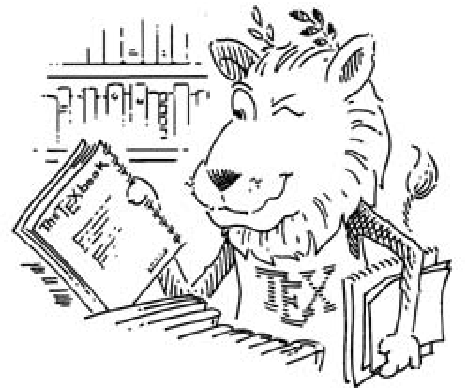
\includegraphics[width=\textwidth]{figuras/lion.pdf}
        \caption{O mascote estudando}\label{fig:mascote1}
    \end{subfigure}
    \begin{subfigure}[t]{.4\textwidth}
        \centering
        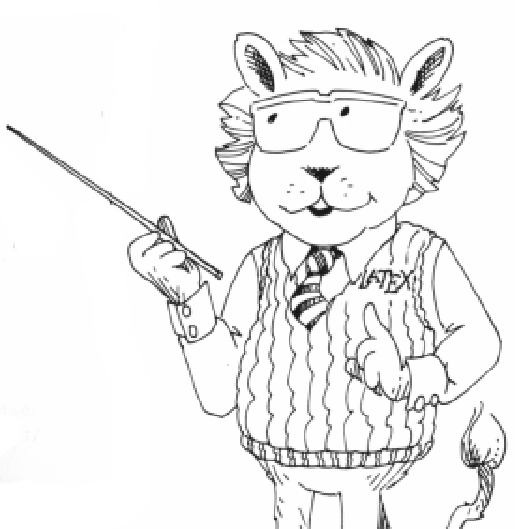
\includegraphics[width=\textwidth]{figuras/latex_lion.pdf}
        \caption{O mascote ensinando}\label{fig:mascote2}
    \end{subfigure}
\end{figure}
\chapter{Proposta}\label{cap:proposta}


\section{Incluindo trechos de códigos}\label{sec:codigos}

Em alguns casos é desejado incluir trechos de códigos no documento. O \LaTeX oferece inúmeras maneiras para isto e o pacote \textbf{listings} é conhecido por apresentar um dos melhores resultados. A \autoref{l_olamundo} apresenta o código em \textit{shell script} para o complexo problema do ``Olá mundo!''. A \autoref{l_matlab} apresenta um trecho de código em MatLab e por fim, na \autoref{cod:pessoa} é ilustrado um aluno representado em um documento \gls{json}.

\lstinputlisting[style=shell,caption={Olá mundo em shell script},label=l_olamundo]{codigos/ola.sh}

\lstinputlisting[style=matlab,caption={Um pequeno código em MatLab},label=l_matlab]{codigos/matlab.m}

\lstinputlisting[style=json,caption={Aluno representado em JSON},label=cod:pessoa]{codigos/pessoa.json}


\section{Como apresentar equações}\label{sec:equacoes}

O \LaTeX é um pacote feito para a preparação de textos impressos de alta qualidade, especialmente
para textos matemáticos. Ele foi desenvolvido por Leslie Lamport a partir do programa~\TeX~criado por Donald Knuth.

Fórmulas matemáticas são produzidas digitando no arquivo fonte texto descrevendo-as. Isto significa que o~\LaTeX~deve ser informado que o texto que vem a seguir é uma fórmula e também quando ela termina e o texto normal recomeça. As fórmulas podem ocorrer em uma linha de texto como $ ax^2 + bx + c = 0 $, ou destacada do texto principal como os exemplos apresentados na \autoref{e_c2_eq1} e \autoref{e_c2_eq2}.

\begin{equation}
 x=\frac{-b\pm\sqrt{b^2-4ac}}{2a}
\label{e_c2_eq1}
\end{equation}

\begin{align}
f(x) &= x^2 \nonumber\\
g(x) &= \dfrac{1}{\sqrt{x}} \nonumber\\
F(x) &= \int^a_b \frac{1}{3}x^3
\label{e_c2_eq2}
\end{align}

\section{Usando siglas, abreviaturas e símbolos}

Algumas vezes nos deparamos com textos cheios de siglas ou símbolos. Existem diversos pacotes e formas para gerar glossário, lista de acrônimos, lista de símbolos etc. com \LaTeX. Neste parágrafo é feito uso de comandos definidos no pacote \textit{glossaries-extra}\footnote{\url{https://www.ctan.org/pkg/glossaries-extra}}. A listagem de acrônimos fica dentro do arquivo \texttt{capitulos/acronimos.tex} e a listagem de símbolos fica dentro do arquivo \texttt{capitulos/simbolos.tex}.

O símbolo \gls{emptyset} representa um conjunto vazio, já o símbolo \gls{pi} representa o número Pi. O protocolo \gls{TLS} deve ser empregado sempre que se deseja garantir a integridade e a confidencialidade das mensagens trocadas pela rede. O \gls{TLS} é hoje utilizado por diversas aplicações. Como faz tempo que eu não falo do \glsxtrfull{TLS} eu chamo o nome completo mais a sigla, ajudando o meu leitor a lembrar da sigla \glsxtrshort{TLS}. Existem as \glsxtrfullpl{AC} que são bem importante. Este documento segue as normas da \gls{ABNT} e para isso faz uso do pacote \gls{abnTeX}.

Abaixo são apresentados os comandos providos pelo pacote \textit{glossaries-extra}:

\begin{itemize}
    \item \verb+\gls{rotulo}+ -- Na primeira vez que o acrônimo for chamado será impresso o valor por extenso e o acrônimo. Ex: \verb+\gls{IFSC}+ irá imprimir Instituto Federal de Santa Catarina (IFSC). Nas demais vezes irá imprimir somente o acrônimo;
    \item \verb+\glspl{rotulo}+ -- Semelhante ao anterior, mas imprime a forma no plural;
    \item \verb+\glsxtrshort{rotulo}+ -- Para imprimir somente o acrônimo;
    \item \verb+\glsxtrlong{rotulo}+ -- Para imprimir somente o valor por extenso;
    \item \verb+\glsxtrfull{rotulo}+ -- Para imprimir o valor por extenso e o acrônimo, mesmo que o acrônimo já tenha sido invocado previamente.
\end{itemize}



\section{Referências bibliográficas}\label{sec:referencias}

A formatação das referências bibliográficas conforme as regras da ABNT são um dos principais objetivos do \abnTeX. Consulte os manuais \citeonline{abntex2cite} e \citeonline{abntex2cite-alf} para obter informações sobre como utilizar as referências bibliográficas.


O uso de citações ao londo do texto é uma prática desejável. Por exemplo, em \cite{lamport94} é apresentado um documento sobre a preparação de textos usando \LaTeX. Já em \cite{goossens94} é apresentada uma lista de referências rápidas para realizar as mais simples tarefas em \LaTeX.

É o caso em que você menciona \emph{explicitamente} o autor da referência na sentença, algo
do tipo ``Fulano (1900)''. Neste caso o nome do autor é escrito
normalmente. Para isso use o comando \verb+\citeonline+.

A ironia será assim uma \ldots\ proposta  por \citeonline{lamport94}. Em \cite{exemplo} foi usado para ilustrar como uma \textit{URL} deve aparecer na seção das referências. Este documento segue as normas da \gls{ABNT} e para isso faz uso do pacote \gls{abnTeX}.


% ---
\section{Citações diretas}
\label{sec-citacao}
% ---

\index{citações!diretas}Utilize o ambiente \texttt{citacao} para incluir
citações diretas com mais de três linhas:

\begin{citacao}
As citações diretas, no texto, com mais de três linhas, devem ser
destacadas com recuo de 4 cm da margem esquerda, com letra menor que a do texto
utilizado e sem as aspas. No caso de documentos datilografados, deve-se
observar apenas o recuo \cite[5.3]{NBR10520:2002}.
\end{citacao}

Use o ambiente assim:

\begin{verbatim}
\begin{citacao}
As citações diretas, no texto, com mais de três linhas [\ldots] 
deve-se observar apenas o recuo \cite[5.3]{NBR10520:2002}.
\end{citacao}
\end{verbatim}

O ambiente \texttt{citacao} pode receber como parâmetro opcional um nome de
idioma previamente carregado nas opções da classe. Nesse
caso, o texto da citação é automaticamente escrito em itálico e a hifenização é
ajustada para o idioma selecionado na opção do ambiente. Por exemplo:

\begin{verbatim}
\begin{citacao}[english]
Text in English language in italic with correct hyphenation.
\end{citacao}
\end{verbatim}

Tem como resultado:

\begin{citacao}[english]
Text in English language in italic with correct hyphenation.
\end{citacao}

\index{citações!simples}Citações simples, com até três linhas, devem ser
incluídas com aspas. Observe que em \LaTeX as aspas iniciais são diferentes das
finais: ``Amor é fogo que arde sem se ver''.


\chapter{Conclusões}\label{cap:conclusoes}

Este trabalho procurou mostrar como deverá ser a apresentação da monografia a ser submetida à Coordenação do Curso de Engenharia de Telecomunicações do \gls{IFSC} para a obtenção do diploma de Bacharel em Engenharia de Telecomunicações.

No \autoref{cap:introducao} foi feita uma pequena introdução. No \autoref{cap:revisao} foi apresentado o uso de alguns ambientes flutuantes no~\LaTeX~. E no \autoref{cap:proposta} foi apresentado sobre equações e como inserir trechos de código.

Como trabalho futuro, fica a reescrita do texto deste documento de forma que ele possam indicar informações específicas a formatação do documento. Como o tamanho da fonte utilizada, o espaçamento da borda, o alinhamento e numeração das seções e capítulos etc.



%-----------------------------------------------%
% ELEMENTOS PÓS-TEXTUAIS
%-----------------------------------------------%
\postextual
% %-----------------------------------------------%
%-----------------------------------------------%
% Referências bibliográficas
%-----------------------------------------------%
\bibliography{referencias}


%-----------------------------------------------%
% Apêndices
%-----------------------------------------------%
\begin{apendicesenv}
% Imprime uma página indicando o início dos apêndices
\partapendices

\chapter{Meu primeiro apêndice}

Texto ou documento, elaborado pelo autor, a fim de complementar sua argumentação, sem prejuízo da unidade nuclear do trabalho. Os apêndices são identificados por letras maiúsculas ordenadas alfabeticamente, travessão e pelo respectivo título. 

\end{apendicesenv}

%-----------------------------------------------%
% Anexos
%-----------------------------------------------%
\begin{anexosenv}
% Imprime uma página indicando o início dos anexos
\partanexos

\chapter{Meu primeiro assunto de anexo}

Texto ou documento não elaborado pelo autor, que serve de fundamentação, comprovação e ilustração. Os anexos são identificados por letras maiúsculas ordenadas alfabeticamente, travessões e pelos respectivos títulos. 


\chapter{Segundo assunto que pesquisei}
\lipsum[31]

\end{anexosenv}


    
\end{document}

